\documentclass{article}
\ProvidesPackage{format}
%Page setup
\usepackage[utf8]{inputenc}
\usepackage[margin=0.7in]{geometry}
\usepackage{parselines} 
\usepackage[english]{babel}
\usepackage{fancyhdr}
\usepackage{titlesec}
\hyphenpenalty=10000

\pagestyle{fancy}
\fancyhf{}
\rhead{Sam Robbins}
\rfoot{Page \thepage}

%Characters
\usepackage{amsmath}
\usepackage{amssymb}
\usepackage{gensymb}
\newcommand{\R}{\mathbb{R}}

%Diagrams
\usepackage{pgfplots}
\usepackage{graphicx}
\usepackage{tabularx}
\usepackage{relsize}
\pgfplotsset{width=10cm,compat=1.9}
\usepackage{float}

%Length Setting
\titlespacing\section{0pt}{14pt plus 4pt minus 2pt}{0pt plus 2pt minus 2pt}
\newlength\tindent
\setlength{\tindent}{\parindent}
\setlength{\parindent}{0pt}
\renewcommand{\indent}{\hspace*{\tindent}}

%Programming Font
\usepackage{courier}
\usepackage{listings}
\usepackage{pxfonts}

%Lists
\usepackage{enumerate}
\usepackage{enumitem}

% Networks Macro
\usepackage{tikz}


% Commands for files converted using pandoc
\providecommand{\tightlist}{%
	\setlength{\itemsep}{0pt}\setlength{\parskip}{0pt}}
\usepackage{hyperref}

% Get nice commands for floor and ceil
\usepackage{mathtools}
\DeclarePairedDelimiter{\ceil}{\lceil}{\rceil}
\DeclarePairedDelimiter{\floor}{\lfloor}{\rfloor}

% Allow itemize to go up to 20 levels deep (just change the number if you need more you madman)
\usepackage{enumitem}
\setlistdepth{20}
\renewlist{itemize}{itemize}{20}

% initially, use dots for all levels
\setlist[itemize]{label=$\cdot$}

% customize the first 3 levels
\setlist[itemize,1]{label=\textbullet}
\setlist[itemize,2]{label=--}
\setlist[itemize,3]{label=*}

% Definition and Important Stuff
% Important stuff
\usepackage[framemethod=TikZ]{mdframed}

\newcounter{theo}[section]\setcounter{theo}{0}
\renewcommand{\thetheo}{\arabic{section}.\arabic{theo}}
\newenvironment{important}[1][]{%
	\refstepcounter{theo}%
	\ifstrempty{#1}%
	{\mdfsetup{%
			frametitle={%
				\tikz[baseline=(current bounding box.east),outer sep=0pt]
				\node[anchor=east,rectangle,fill=red!50]
				{\strut Important};}}
	}%
	{\mdfsetup{%
			frametitle={%
				\tikz[baseline=(current bounding box.east),outer sep=0pt]
				\node[anchor=east,rectangle,fill=red!50]
				{\strut Important:~#1};}}%
	}%
	\mdfsetup{innertopmargin=10pt,linecolor=red!50,%
		linewidth=2pt,topline=true,%
		frametitleaboveskip=\dimexpr-\ht\strutbox\relax
	}
	\begin{mdframed}[]\relax%
		\centering
		}{\end{mdframed}}



\newcounter{lem}[section]\setcounter{lem}{0}
\renewcommand{\thelem}{\arabic{section}.\arabic{lem}}
\newenvironment{defin}[1][]{%
	\refstepcounter{lem}%
	\ifstrempty{#1}%
	{\mdfsetup{%
			frametitle={%
				\tikz[baseline=(current bounding box.east),outer sep=0pt]
				\node[anchor=east,rectangle,fill=blue!20]
				{\strut Definition};}}
	}%
	{\mdfsetup{%
			frametitle={%
				\tikz[baseline=(current bounding box.east),outer sep=0pt]
				\node[anchor=east,rectangle,fill=blue!20]
				{\strut Definition:~#1};}}%
	}%
	\mdfsetup{innertopmargin=10pt,linecolor=blue!20,%
		linewidth=2pt,topline=true,%
		frametitleaboveskip=\dimexpr-\ht\strutbox\relax
	}
	\begin{mdframed}[]\relax%
		\centering
		}{\end{mdframed}}
\lhead{Programming Paradigms - Systems Programming}
\usepackage{boxedminipage}
\usetikzlibrary{shapes.misc}
\usetikzlibrary{shapes.geometric, arrows, positioning}
\usepackage{minted}

\begin{document}
	\begin{center}
		\underline{\huge UNIX and C}
	\end{center}

\section{The Shell}
\begin{itemize}
\item A powerful way to perform work on a computer through a text interface
\begin{itemize}
\item Run programs
\item Control how the programs work
\end{itemize}
\item Perform sequences of commands to achieve even more complex work
\item There are many choices for which shell to use, the most popular of which is \verb!bash! (bourne again shell)
\end{itemize}



\section{Ethos of the UNIX Shell}
\begin{itemize}
\item Not one monolithic program
\item Instead many small programs
\item Allow user to combine these together to make new functionality
\begin{itemize}
\item Using pipes
\item Using script files
\end{itemize}
\end{itemize}



\section{\texttt{stdin}, \texttt{stdout} and \texttt{stderr}}
\begin{itemize}
\item Remove the need to worry about I/O devices
\item Two types of output, each can be redirected
\item These are stream variables, can redirect e.g. \verb!2>&1!
\end{itemize}
\begin{center}
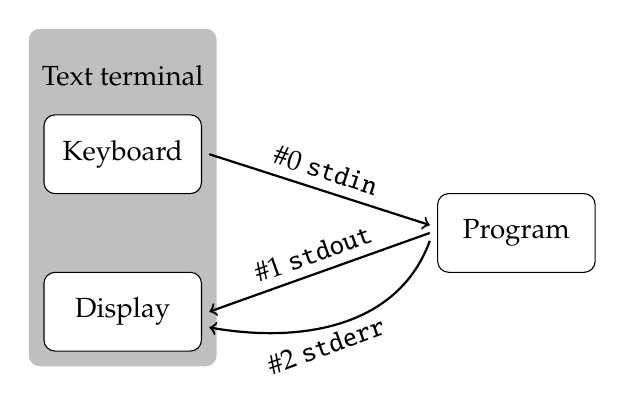
\begin{tikzpicture}
\draw [white] (4.9,-1.2) -- (2.1,-2.2) node[midway, sloped, below, black] {\#2 \texttt{stderr}};
\draw[rounded corners, color=white, fill=lightgray] (-0.2, -2.2) rectangle (2.2, 2.1) {};
\node at (1,1.5) {Text terminal};
\draw[rounded corners,fill=white] (0, 0) rectangle (2, 1) {};
\node at (1,0.5) {Keyboard};
\draw [thick, ->] (2.1,0.5) -- (4.9,-0.4) node[midway, sloped, above] {\#0 \texttt{stdin}};
\draw[rounded corners, fill=white] (0, -1) rectangle (2, -2) {};
\node at (1,-1.5) {Display};
\draw [thick, ->] (4.9,-0.5) -- (2.1,-1.5) node[midway, sloped, above] {\#1 \texttt{stdout}};
\draw [thick, ->] (4.9,-0.6) to[out=250, in=350] (2.1,-1.7) {};
\draw[rounded corners, fill=white] (5, -1) rectangle (7, 0) {};
\node at (6,-0.5) {Program};
\end{tikzpicture}
\end{center}



\section{Pipes}
\begin{itemize}
\item The shell provides you with many small `tools'
\begin{itemize}
\item The power comes from composing them together
\item Pipes provide a means to do this
\item Each command takes input (from the keyboard)
\item Each command produces output (to the screen)
\end{itemize}
\item We can redirect input or output
\begin{itemize}
\item \verb!<! take input from a file
\item \verb!>! write output to a file
\item \verb!|! take the output of one command and use as input to next
\end{itemize}
\end{itemize}



\section{Output pipes}
\begin{itemize}
\item Add ``\verb!>!'' or ``\verb!>>!'' and the name of a file after your command before you hit ``Enter/Return'' -- e.g. ``\verb!ps > file.txt!''

\item If the file doesn't exist already, it will be created for you in the directory in which you are working

\item ``\verb!>>!'' appends, ``\verb!>!'' overwrites -- so be careful when using ``\verb!>!''!!
\end{itemize}







\section{\texttt{grep}}
\begin{itemize}
\item \verb!grep! is a search tool that uses regular expressions for matching
\begin{itemize}
\item \mintinline{bash}{grep "help" file.txt}
\begin{itemize}
\item Lists all lines in \verb!file.txt! containing the word `\verb!help!'
\end{itemize}
\end{itemize}
\end{itemize}



\section{Regular Expressions}
\begin{itemize}
\item A concise way to match different strings
\begin{itemize}
\item \verb!*! - match any number of the proceeding character
\item \verb!?! - match one of the proceeding character
\item \verb!+! - match one or more of the proceeding character
\item \verb![ABC]! - class as single character
\item \verb![A-Z]! - all the upper case characters \verb!A! to \verb!Z!
\end{itemize}
\item e.g. \verb![A-Za-z]*[0-9].txt!
\end{itemize}



\section{\texttt{sort}}
\begin{itemize}
\item Sorts a file (if specified)
\begin{itemize}
\item \verb!stdin!: standard input, by default from terminal
\end{itemize}
\item Where does it put the results? 
\begin{itemize}
\item \verb!stdout!: standard output, by default the terminal
\item or a file with \verb!-o filename!
\end{itemize}
\end{itemize}



\section{\texttt{tr} - translate}
\begin{itemize}
\item \verb!tr SET1 SET2!
\begin{itemize}
\item translates or deletes characters from \verb!SET1! to \verb!SET2!
\item e.g. \verb!tr 'A-Z' 'a-z'! makes a lower case version of \verb!stdin!
\item option \verb!-c! takes complement of \verb!SET1!
\item option \verb!-s! squeezes repeats to a single character
\item option \verb!-d! deletes all characters in \verb!SET1!
\item e.g. \verb!tr -dc '[:print:]'! - deletes all non printable characters
\end{itemize}
\end{itemize}



\section{Options and more options\ldots}
\begin{itemize}
\item Most UNIX commands have many options
\item To find out what these are:
\begin{itemize}
\item Ask the command
\begin{itemize}
\item e.g. \verb!sort --help!, \verb!grep -h!
\end{itemize}
\item Refer to the manual
\begin{itemize}
\item e.g. \verb!man sort!, \verb!man tr!
\end{itemize}
\item Go online
\begin{itemize}
\item e.g. Search command in Google
\end{itemize}
\end{itemize}
\end{itemize}



\section{\texttt{uniq}}
\begin{itemize}
\item Remove or report repeated lines
\item Use with \verb!sort! to find lines repeated throughout document
\item e.g. \verb!sort | uniq!
\item Use \verb!-c! option to count number of repetitions
\item Tie these all together: what does this do?
\item 
\begin{minted}{bash}
tr 'A-Z' 'a-z' < infile | tr -cs 'a-z' '\n' | sort \
      | uniq -c | sort -n!
\end{minted}
\end{itemize}



\section{Defining our own UNIX command}
\begin{itemize}
\item UNIX commands are just executables, most of which are written in C
\item Suppose we want to count only frequent words, we could write a filter function to forward lines starting with a number above a certain value
\end{itemize}



\begin{minted}{c}
#include <stdio.h>

int main(int argc, char* argv[]){

  int limit;
  sscanf(argv[1], "%d", &limit);

  char* line = NULL;
  size_t size=0;
  while(getline(&line, &size, stdin) >0){
    int number = 0;
    sscanf(line,"%d", &number);
    if(number>= limit){
      printf("%s", line);
    }
  }
return 0;
}
\end{minted}



\section{Formatting (\texttt{stdio.h})}
{\renewcommand{\arraystretch}{2}
\begin{tabularx}{\textwidth}{|X|X|}
\hline
\texttt{printf(char *format, ...)} & To \texttt{stdout}\\
\hline
\texttt{fprintf(FILE *stream, char *format, ...)}&To file/stream specified\\
\hline
\texttt{sprintf(char *str, char *format, ...)}&
\begin{itemize}
	\item Write into string/array specified 
	\item String needs memory to be allocated already
\end{itemize}\\
\hline
\texttt{scanf(char *format,...)}& From \texttt{stdin} to specified variables\\
\hline
\texttt{fscanf(FILE *stream, char *format,...)}&
\begin{itemize}
	\item From specified file 
	\item \texttt{scanf(...)} is the same as \texttt{fscanf(stdin,...)}
\end{itemize}\\
\hline
\texttt{sscanf(char *str,char *format,...)}&From a given string\\
\hline


\end{tabularx}
}


\section{\texttt{getline()}}
\begin{itemize}
\item From GNU C lib and is more reliable than \verb!gets()!
\item Parameters
\begin{itemize}
\item Pointer to \verb!malloc()!'d block for result
\begin{itemize}
\item will \verb!malloc()! if \verb!NULL!
\end{itemize}
\item Pointer for number of bytes in the \verb!malloc()!'d block
\item Stream to read from
\end{itemize}
\end{itemize}



\section{Using our program in UNIX}
\begin{itemize}
\item Compile: \verb!gcc filter.c -o filter!
\item Put in a pipe e.g.
\begin{minted}{bash}
tr 'A-Z' 'a-z' < filter.c | tr -cs 'a-z' '\n' \
       | sort | uniq -c | sort -n | ./filter 3

wc * | sort -n | ./filter 10
\end{minted}
\end{itemize}



\section{Be robust}
\begin{itemize}
\item Check the number of command line parameters
\item Report problems to \verb!stderr!
\item Return value of \verb!main()!
\item For more complex joining of UNIX commands use shell script
\end{itemize}



\section{File handling}
\begin{itemize}
\item Files are stored in a hierarchical structure
\item Allows grouping
\item Navigation
\begin{itemize}
\item \verb!ls! - list the current folder
\item \verb!cd! - change folder
\item \verb!mkdir! - make new folder
\item \verb!mv! - move a file / folder
\item \verb!cp! - copy a file / folder
\item \verb!rm! - delete a file
\item \verb!rmdir! - delete a folder
\item \verb!du! - how much space does a folder / file take?
\item \verb!find! - list all files
\end{itemize}
\end{itemize}

\section{Shell scripts}
\begin{itemize}
\item A Shell Script is simply a collection of commands enclosed in a file
\item Useful for when you have to type lots of commands to do one thing
\item Whilst this is not impossible, it can get rather time-consuming
\item Putting all the commands into a shell script enables them to be executed at the command line in one single command
\end{itemize}



\section{Writing a Shell Script}
\begin{itemize}
\item You can write shell scripts in any text editor of your choosing

\item They should be saved with a \verb!.sh! extension, e.g. \verb!myscript.sh!

\item They must all begin with the line \verb~#!/bin/bash~
\begin{itemize}
\item ``\verb~#!~'' tells UNIX this is a script that can be run
\item \verb!/bin/bash! tells Linux what program to run the script with
\end{itemize}
\end{itemize}



\section{Example}
\begin{itemize}
\item This script creates a new directory, changes into it and creates two new text files
\begin{minted}{c}
#!/bin/bash
mkdir newDirectory
cd newDirectory
touch file1.txt
touch file2.txt 
\end{minted}
\end{itemize}



\section{How do you run a shell script?}
\begin{itemize}
\item Firstly, you need to make sure you have permission to execute the script file
Use the \verb!chmod! command to do this
\begin{itemize}
\item \verb!chmod a+x myscript.sh!
\end{itemize}

\item Then, at the command line, type \verb!./scriptname! and your script should run
\begin{itemize}
\item e.g. \verb!./myscript.sh!
\end{itemize}
\end{itemize}



\section{Doing things to multiple files}
\begin{itemize}
\item A handy little tool for doing the same operation to lots of files
\begin{minted}{bash}
#!/bin/bash
for f in *
do
  #something in here
  echo $f
done
\end{minted}
\end{itemize}



\section{Parameters}
\begin{itemize}
\item You can add parameters to a script when you run them
\item \verb!./myscript.sh foo bar!
\begin{itemize}
\item ``\verb!foo!'' and ``\verb!bar!'' are the parameters here
\end{itemize}

\item Refer to them using the \verb!$! sign in scripts
\begin{itemize}
\item \verb!$1!, \verb!$2!, etc.
\end{itemize}
\end{itemize}



\section{The \texttt{if} statement in shell scripts}
\begin{minted}{c}
#!/bin/bash
if [ $1 -lt $2 ] 
then
  echo "yes" $1 "is less than" $2
else 
  echo "no it isn't"
fi
\end{minted}
\begin{itemize}
\item The \verb!else! bit is optional
\item Uses \verb!==!, \verb~!=~, \verb!-gt!, \verb!-lt!, \verb!-le!, \verb!-ge! for equality, inequality, greater than, less than, less than or equal, greater than or equal
\end{itemize}



\section{Some last bits}
\begin{itemize}
\item \verb!if [ -a FILE ]! - true if \verb!FILE! exists
\item \verb!if [ -z STRING ]! - true if \verb!STRING! is empty
\item Variables:
\begin{itemize}
\item \verb!VAR="Hello World"!
\item \verb!echo $VAR!
\item \verb!TD="The time is `date`"!
\item \verb!echo $TD!
\begin{itemize}
\item \verb!The time is Wed 20 Nov 15:44:14 GMT 2019!
\end{itemize}
\end{itemize}
\end{itemize}






\end{document}
